
%(BEGIN_QUESTION)
% Copyright 2007, Tony R. Kuphaldt, released under the Creative Commons Attribution License (v 1.0)
% This means you may do almost anything with this work of mine, so long as you give me proper credit

The {\it activated sludge} process exploits the natural decomposing action of bacteria to digest organic compounds dissolved and suspended in wastewater.  These compounds precipitate more easily after being digested by the bacteria, and are removed from the water as sludge through clarification and settling.

In order for the activated sludge process to work well, bacteria must be supplied with an ample amount of air, and a constant stream of bacteria-laden (``activated'') sludge must be re-introduced into the aeration chamber to maintain a culture capable of continually digesting incoming waste.

Examine the following P\&ID, and explain how the instruments help ensure proper ``care and feeding'' of the bacteria for good operation:

$$\includegraphics[width=15.5cm]{i01809x01.eps}$$

\vskip 20pt \vbox{\hrule \hbox{\strut \vrule{} {\bf Suggestions for Socratic discussion} \vrule} \hrule}

\begin{itemize}
\item{} Identify whether the flow controller needs to be {\it direct} or {\it reverse} acting.
\item{} For those who have already studied flowmters, explain why a {\it magnetic} flowmeter is ideally suited for measuring sludge flow, where the sludge has the approximate consistency (and appearance!) of peanut butter.
\item{} For those who have already studied flowmeters, identify the flowmeter type used to measure influent flow and also explain why it has a square-root symbol next to it.
\item{} Explain what a {\it clarifier} vessel does, and the purposes each one serves in this process.
\item{} Explain what will happen in this system if the venturi tube flowmeter fails with a low signal.
\item{} Explain what will happen in this system if the venturi tube flowmeter fails with a high signal.
\item{} Explain what will happen in this system if the magnetic flowmeter fails with a low signal.
\item{} Explain what will happen in this system if the magnetic flowmeter fails with a high signal.
\end{itemize}

\underbar{file i01809}
%(END_QUESTION)





%(BEGIN_ANSWER)

Both air and activated sludge flow rates to the aerator are controlled in accordance with the flow rate of the incoming wastewater (discharged from the primary clarifier).  A low limit relay maintains a minimum flow rate of air into the aerator to maintain an aerobic bacterial culture and to prevent sludge from compacting at the bottom during periods of low wastewater flow.

%(END_ANSWER)





%(BEGIN_NOTES)

\vfil \eject

\noindent
{\bf Summary Quiz:}

Suppose the influent flowmeter in this activated sludge water treatment system fails with a low (0\%) output signal:

$$\includegraphics[width=15.5cm]{i01809x02.eps}$$

What effects will this fault have on the actual sludge flow rate and air flow rate into the aeration chamber?

\begin{itemize}
\item{} Sludge flow maintains at 10\% ; air flow maintains at 10\% 
\vskip 5pt 
\item{} Sludge flow maintains at 10\% ; air flow stops
\vskip 5pt 
\item{} Sludge flow maintains at 50\% ; air flow maintains at 50\%
\vskip 5pt 
\item{} Sludge flow stops ; air flow stops
\vskip 5pt 
\item{} Sludge flow stops ; air flow maintains at 10\%
\vskip 5pt 
\item{} Sludge flow goes to 100\% ; air flow goes to 100\%
\end{itemize}



%INDEX% Control, strategies: ratio
%INDEX% Process: activated sludge wastewater treatment

%(END_NOTES)


